\documentclass{ieeeaccess}
\usepackage{cite}
\usepackage{amsmath,amssymb,amsfonts}
\usepackage{amsthm}
\usepackage{algorithmic}
\usepackage{algorithm}
\usepackage{graphicx}
\usepackage{textcomp}

\usepackage{booktabs}
\usepackage{multirow}
\usepackage{hyperref}
\usepackage{pifont}
\usepackage{tikz}
\usetikzlibrary{shapes,arrows,positioning,fit,calc}
\usepackage{subcaption}
\usepackage{enumitem}
\usepackage{url}


\newtheorem{theorem}{Theorem}
\newtheorem{proposition}{Proposition}
\newtheorem{assumption}{Assumption}

\begin{document}
\history{Date of publication xxxx 00, 0000, date of current version xxxx 00, 0000.}
\doi{10.1109/ACCESS.2026.XXXXXXX}

\title{HMARL-SOC: Hierarchical Multi-Agent Reinforcement Learning for Autonomous Security Operations Center Coordination}

\author{\uppercase{Nutthakorn Chalaemwongwan}\authorrefmark{1}}
\address[1]{Department of Computer Engineering, KOSEN-KMITL, King Mongkut's Institute of Technology Ladkrabang, Bangkok, Thailand (e-mail: nutthakorn.ch@kmitl.ac.th)}

\markboth
{Chalaemwongwan: HMARL-SOC}
{Chalaemwongwan: HMARL-SOC}

\corresp{Corresponding author: Nutthakorn Chalaemwongwan (e-mail: nutthakorn.ch@kmitl.ac.th).}

\begin{abstract}
Enterprise Security Operations Centers (SOCs) routinely face thousands of security events per hour, yet analysts can resolve fewer than half within a shift. We present HMARL-SOC, a three-tier hierarchical multi-agent reinforcement learning architecture that mirrors the division of labor in real SOC teams. A Strategic Coordinator (PPO) decomposes campaign-level threats into sub-tasks for three operational agents: proactive threat hunting (SAC), alert triage and correlation (DQN), and coordinated incident response (MADDPG). The system is formalized as a Dec-POMDP integrating SIEM, EDR, and SOAR tool APIs, trained with a four-term reward covering detection, response speed, disruption cost, and false positive penalty. On a 200-host MITRE ATT\&CK simulator with 5-phase campaigns, HMARL-SOC achieves the lowest false positive rate (0.17\%, $p{<}0.001$ vs.\ QMIX) and the highest cumulative reward (+6.9), which captures the best balance across all four objectives, at 71.0\% containment success. Per-step cost is $O(N{\cdot}d^2)$ ($N$ agents, observation dimension $d$), enabling real-time inference at 4.2\,ms per decision step on 200 hosts. Ablation studies confirm that every architectural component---the Strategic Coordinator, shared replay buffer, and heterogeneous RL algorithms---contributes measurably to overall performance. Cross-environment transfer to CybORG CAGE Challenge~4 demonstrates that the learned hierarchical structure generalizes beyond the training simulator. Code available at: \url{https://github.com/nutthakorn7/HMARL-SOC}. This paper is an extended version of our conference paper presented at ITC-CSCC 2026~\cite{conf_version}.
\end{abstract}

\begin{keywords}
Multi-Agent Reinforcement Learning, Threat Hunting, Incident Response, Security Operations Center, Deep Reinforcement Learning, Cybersecurity, Hierarchical Reinforcement Learning
\end{keywords}

\titlepgskip=-21pt

\maketitle

\section{Introduction}
\label{sec:introduction}
\PARstart{O}{n} any given shift, a mid-sized enterprise SOC might ingest anywhere from 5,000 to 50,000 security events per hour---the bulk of them flowing out of SIEM, EDR, and cloud telemetry pipelines. Buried somewhere in that volume are the few events that actually matter, and analysts have to find them while simultaneously coordinating containment across network segments that often run entirely different stacks~\cite{b1}. The pressure is only growing: Gartner projected that 75\% of SOCs would adopt some form of AI-driven analyst assistant by 2026~\cite{b2}, and the CAGE Challenge 4~\cite{b24} already benchmarks multi-agent policies against enterprise-scale attack scenarios.

In practice, the SOC workflow comprises not one job but three distinct functions. Threat hunters look for hypothesis-driven indicators of compromise in endpoint logs that automated tools would miss. Meanwhile, alert triage analysts sort and bucket alerts so that responders are not chasing the same issue. Finally, incident responders take action: pushing firewall rules, containing compromised endpoints, and extracting forensics. And, importantly, these three jobs interact. Hunters enable triagers. Triage influences which alerts, if any, the responder will resolve. Yet, surprisingly, existing RL approaches to this problem almost never model this interaction~\cite{b3,b4}.

Beyond these gaps, a survey of cyber defense RL literature reveals three additional shortcomings. Threat hunting and incident response have never before been modeled as related optimization problems~\cite{b7}. Single-agent models try to pack too much into a single policy that is expected to reflect the expertise of three distinct roles. Flat multi-agent models like independent Q-learning are closer to the right conceptualization, however---they fail to capture the hierarchical structure of multi-stage attacks that demand a unified, coordinated response.

HMARL-SOC (\textbf{H}ierarchical \textbf{M}ulti-\textbf{A}gent \textbf{R}einforcement \textbf{L}earning for \textbf{SOC} operations) addresses all three gaps. This paper extends our conference publication~\cite{conf_version} with the following additional contributions:
\begin{enumerate}[leftmargin=*, nosep]
    \item A \textbf{Dec-POMDP formalization} that wires threat hunting observations directly into incident response actions via SOC tool interfaces, rather than treating them as separate MDPs.
    \item A \textbf{three-tier agent hierarchy} that mirrors how SOC teams are actually organized: a strategic coordinator trained with PPO on top, and three operational agents underneath, each using the RL algorithm best suited to its action space (SAC, DQN, and MADDPG respectively).
    \item A \textbf{composite reward function} whose four weighted terms---detection coverage, response latency, operational disruption, and false-positive cost---let practitioners dial in their own risk appetite.
    \item An \textbf{empirical evaluation} on a 200-host, 5-segment MITRE ATT\&CK simulator, benchmarked against five baselines including QMIX and MAPPO.
    \item \textbf{[NEW]} A comprehensive \textbf{ablation study} quantifying the contribution of each architectural component: Strategic Coordinator, shared replay buffer, and heterogeneous RL algorithms.
    \item \textbf{[NEW]} A \textbf{scalability analysis} with wall-clock benchmarks from 50 to 500 hosts demonstrating linear scaling.
    \item \textbf{[NEW]} A \textbf{CybORG CAGE-4 zero-shot transfer study} demonstrating that the learned hierarchical structure generalizes to an unseen environment.
    \item \textbf{[NEW]} Formal \textbf{convergence analysis} with theoretical guarantees for the hierarchical training procedure.
    \item \textbf{[NEW]} A $K$\textbf{-sensitivity analysis} confirming that the temporal abstraction factor $K{=}5$ yields optimal performance across five tested values.
\end{enumerate}

The rest of the paper is laid out as follows. Section~\ref{sec:related} covers related work, Section~\ref{sec:formulation} formalizes the environment and Dec-POMDP, Section~\ref{sec:framework} walks through the HMARL-SOC architecture, Section~\ref{sec:convergence} presents formal convergence analysis, Section~\ref{sec:experiments} presents experiments, Section~\ref{sec:ablation} provides ablation studies, Section~\ref{sec:transfer} discusses cross-environment transfer, Section~\ref{sec:limitations} addresses limitations, and Section~\ref{sec:conclusion} concludes.

%=====================================================================
\section{Related Work}
\label{sec:related}
%=====================================================================

\subsection{RL and MARL for Cybersecurity}
Reinforcement learning has already made its way into some corners of cybersecurity---intrusion detection~\cite{b3}, network defense~\cite{b5}, even automated penetration testing~\cite{b6}. The survey by Nguyen and Reddi~\cite{b4} maps out the DRL body of work for cybersecurity and singles out autonomous cyber defense as an expansion area of interest; Foley et al.~\cite{b11,b25} later cast it in practical terms. On incident response in particular, the ARCS framework~\cite{b7} demonstrated that DRL can accelerate containment decisions---but only under a single-agent model that collapses when network complexity rises. When we have multiple decision-makers, the next logical step up is Multi-Agent RL~\cite{b8}. Hierarchical variants are scalable~\cite{b9}, and the CAGE Challenge 4~\cite{b24} has committed the community to an enterprise-scale evaluation. There are two studies of particular interest to ours. Singh et al.~\cite{b26} cast autonomous cyber defense as a hierarchical MARL policy structure that decomposes the problem into investigation and recovery sub-policies and validates on the CybORG platform. Alshamrani~\cite{b27} goes further with AZH-MARL, which adds a layer of zero-shot generalization and federated knowledge graph sharing on top of a hierarchical model, yielding 94.2\% detection of known attacks. But all of these studies target network defense mechanisms only---compromised host clean-up, malicious traffic filtering---and ignore the SOC workflow that connects threat hunting, alert processing and incident response into a single operational pipeline. Table~\ref{tab:comparison} shows the comparison.

\begin{table}[t]
\caption{Comparison with Existing MARL Cyber Defense Approaches}
\label{tab:comparison}
\centering
\scriptsize
\begin{tabular}{lccccc}
\toprule
\textbf{Approach} & \textbf{Unified} & \textbf{SOC} & \textbf{Hetero.} & \textbf{Explain-} \\
 & \textbf{TH+IR} & \textbf{Tools} & \textbf{RL} & \textbf{ability} \\
\midrule
ARCS~\cite{b7} & \ding{55} & \ding{55} & \ding{55} & \ding{55} \\
CAGE-4~\cite{b24} & \ding{55} & \ding{55} & \ding{55} & \ding{55} \\
Singh~\cite{b26} & \ding{55} & \ding{55} & \ding{51} & \ding{55} \\
AZH-MARL~\cite{b27} & \ding{55} & \ding{55} & \ding{55} & \ding{55} \\
\textbf{HMARL-SOC} & \ding{51} & \ding{51} & \ding{51} & \ding{51} \\
\bottomrule
\multicolumn{5}{l}{\scriptsize Criteria reflect SOC-specific features. CAGE-4 and Singh} \\
\multicolumn{5}{l}{\scriptsize also offer public benchmarks; AZH-MARL adds federated learning.} \\
\end{tabular}
\end{table}

\subsection{SOC Automation}
In practice, commercial SOAR platforms encode analyst knowledge as deterministic if-then playbooks---``if the alert severity is high \textbf{and} the source IP sits on a watchlist, isolate the host''~\cite{b13}. These rules do work for the attacks they were written for, but they fail when the attack changes or when the network topology changes, and updating them is manual. There is a newer line of research that applies LLMs to multi-agent pipelines for security analysis~\cite{b14}: the results are encouraging, but this approach is essentially prompt-based and lacks formal convergence properties. In contrast with both lines of work, ours does two things differently. On the action-space side, we attach SOC tool APIs---i.e., SIEM queries, EDR pulls for telemetry data, pushing firewall rules---directly to what agents can execute, so that what is learned maps directly onto a realizable policy executed in the SOC rather than (e.g.) to a fictional ``block host'' command. On the structural side, our three-tier architecture maps onto the operational SOC's current three-tier Tier-1/Tier-2/Tier-3 escalation structure, which makes learned policies more tractable for practitioners to audit and trust.

\subsection{Sim-to-Real Transfer in Cyber RL}
A persistent challenge in applying RL to cybersecurity is the gap between simulated and real-world network environments. Simulation platforms such as CybORG~\cite{b12}, FARLAND~\cite{b29}, and Network Attack Simulator (NASim)~\cite{b30} provide controlled settings for policy training, but their simplified dynamics---deterministic exploits, uniform host configurations, and compressed timescales---inevitably diverge from production networks. Recent work has explored domain randomization~\cite{b31}, progressive neural networks, and curriculum-based transfer to mitigate this gap. In the SOC context, the challenge is amplified by the heterogeneity of tool outputs: a real SIEM produces semistructured logs whose schema varies across vendors, whereas simulators typically emit fixed-length feature vectors. Our CybORG transfer experiment (Section~\ref{sec:transfer}) quantifies this domain gap and demonstrates that the hierarchical coordination structure, rather than the low-level feature representations, is the primary source of transferable knowledge.

\subsection{LLM-Augmented Security Operations}
Large language models have recently been integrated into SOC workflows for alert summarization, playbook generation, and threat intelligence extraction~\cite{b14,b32}. Multi-agent LLM frameworks such as AutoSOC~\cite{b33} assign specialized roles (analyst, responder, coordinator) to LLM instances, achieving promising results on synthetic incident triage benchmarks. However, these systems rely on prompt engineering rather than learned policies and lack formal convergence guarantees; their outputs are also difficult to bound or verify, which raises trust concerns in high-stakes SOC environments. HMARL-SOC and LLM-based approaches are complementary: the former provides principled decision-making with convergence properties (Section~\ref{sec:convergence}), while the latter could serve as a natural-language interface layer on top of the learned policies---a direction we identify in Section~\ref{sec:limitations} as future work.

%=====================================================================
\section{System Model and Problem Formulation}
\label{sec:formulation}
%=====================================================================

\subsection{Enterprise SOC Environment}

We model an enterprise network as a directed graph $\mathcal{G} = (\mathcal{V}, \mathcal{E})$, where vertices $\mathcal{V} = \{v_1, \ldots, v_M\}$ represent network segments (e.g., DMZ, internal subnets, cloud workloads) and edges $\mathcal{E}$ represent connectivity. The security infrastructure comprises a set of tools $\mathcal{T} = \{\text{SIEM}, \text{EDR}, \text{SOAR}, \text{TIP}, \text{Firewall}\}$ that provide observation channels and action interfaces.

At each time step $t$, the environment generates security events $e_t \in \mathcal{F}_{\text{events}}$ from both legitimate operations and adversarial activities. The attacker follows multi-stage campaigns aligned with the MITRE ATT\&CK framework, progressing through phases: Reconnaissance $\rightarrow$ Initial Access $\rightarrow$ Execution $\rightarrow$ Lateral Movement $\rightarrow$ Exfiltration.

\subsection{Dec-POMDP Formulation}

We formalize the SOC defense problem as a Decentralized Partially Observable Markov Decision Process (Dec-POMDP) defined by the tuple:
\begin{equation}
    \mathcal{M} = \langle N, \mathcal{S}, \{\mathcal{A}_i\}_{i=1}^{N}, \{\Omega_i\}_{i=1}^{N}, T, O, R, \gamma \rangle
\end{equation}
where $N$ is the number of agents, $\mathcal{S}$ is the global state space encoding network status and attack progression, $\mathcal{A}_i$ and $\Omega_i$ are agent-specific action and observation spaces, $T: \mathcal{S} \times \mathcal{A} \rightarrow \Delta(\mathcal{S})$ is the transition function, $O: \mathcal{S} \times \mathcal{A} \rightarrow \Delta(\Omega)$ is the observation function, $R: \mathcal{S} \times \mathcal{A} \rightarrow \mathbb{R}$ is the reward function, and $\gamma \in [0,1)$ is the discount factor.

Each agent $i$ maintains a local action-observation history $\tau_i^t = (o_i^1, a_i^1, \ldots, o_i^t)$ and selects actions according to its policy $\pi_i(a_i^t | \tau_i^t)$. The joint policy $\boldsymbol{\pi} = (\pi_1, \ldots, \pi_N)$ maximizes the expected cumulative discounted reward:
\begin{equation}
    J(\boldsymbol{\pi}) = \mathbb{E}\left[\sum_{t=0}^{\infty} \gamma^t R(s_t, \mathbf{a}_t) \;\middle|\; \boldsymbol{\pi}\right]
\end{equation}

\subsection{Observation and Action Spaces}
Each agent receives observations tailored to its role. The Threat Hunter observes network flow statistics, endpoint behavioral features, and threat intelligence feeds ($o_{\text{TH}}^t \in \mathbb{R}^{128}$), with continuous actions controlling investigation depth and scope. The Alert Triage agent observes alert attributes ($o_{\text{AT}}^t \in \mathbb{R}^{64}$) with discrete actions $\{\text{escalate, suppress, correlate, enrich}\}$. The Response Orchestrator observes network state and active incidents ($o_{\text{RO}}^t \in \mathbb{R}^{96}$) with hybrid actions for response type selection and parameterization.

\subsection{Composite Reward Function}
We propose a multi-objective reward function:
\begin{equation}
    R(s_t, \mathbf{a}_t) = \alpha R_{\text{det}} + \beta R_{\text{resp}} + \delta R_{\text{cost}} + \lambda R_{\text{fp}}
\end{equation}
where $R_{\text{det}}$ rewards true positive detections proportional to attack stage severity, $R_{\text{resp}}$ rewards timely containment inversely proportional to elapsed time since detection, $R_{\text{cost}}$ penalizes operational disruption, and $R_{\text{fp}}$ penalizes false positives. The weights $\alpha, \beta, \delta, \lambda$ reflect organizational risk tolerance.

%=====================================================================
\section{Proposed Framework: HMARL-SOC}
\label{sec:framework}
%=====================================================================

\subsection{Hierarchical Architecture}

The HMARL-SOC architecture is a three-tiered (Fig.~\ref{fig:architecture}) architecture, which is intentionally made to reflect the structure of SOC teams in the real world. The tiers are:

\textbf{Tier 1 -- Strategic Coordinator (SC):} The SC is at the top level, where it receives aggregated threat intelligence, the network-wide risk scores for all operational agents beneath it, and the status of all operational agents beneath it. The SC uses this information to factor campaign-level threats into sub-tasks and passes them down as strategic directives $d_t \in \mathcal{D}$ (i.e., priority levels, resource allocation, triage limits, etc.). The SC's meta-policy $\pi_{\text{SC}}$ is trained using Proximal Policy Optimization (PPO)~\cite{b15}, which is a stable algorithm for campaign-level threats despite the noise and delay of the rewards it receives.

\textbf{Tier 2 -- Operational Agents:} Below the SC are three operational agents, each with a different RL algorithm based on the structure of their action spaces:
\begin{itemize}[leftmargin=*, nosep]
    \item \textbf{Threat Hunter (TH):} This agent performs an anytime continuous-action scan of endpoint logs for IOCs and anomalies. Soft Actor-Critic (SAC)~\cite{b16} is a good algorithm for this type of agent, since its entropy bonus encourages the agent to explore all areas of the network that it may encounter (and has the potential to become dangerous), rather than focusing on known patterns of threat behavior.
    
    \item \textbf{Alert Triage (AT):} Alerts received by the system are ranked, grouped and either escalated or terminated. A Deep Q-Network (DQN)~\cite{b17} is suitable for this agent, as it must make discrete classification decisions for each alert that it receives.
    
    \item \textbf{Response Orchestrator (RO):} Once a legitimate threat is identified by the system, this agent is responsible for implementing remediation and containment actions across affected network segments. In this case, Multi-Agent Deep Deterministic Policy Gradient (MADDPG)~\cite{b18} is a good algorithm, as remediation can require multiple agents performing separate but coordinated actions in a specific order to effectively contain the threat.
\end{itemize}

\textbf{Tier 3 -- Communication Layer:} A shared experience replay buffer lets agents learn from each other's transitions, so a discovery by the Threat Hunter can immediately benefit the Response Orchestrator's policy. Layered on top is an attention-based module~\cite{b19} that produces human-readable explanations for each automated decision---a feature that, in our experience, is non-negotiable for any tool meant to operate inside a real SOC.

\begin{figure}[t]
    \centering
    \resizebox{\columnwidth}{!}{%
    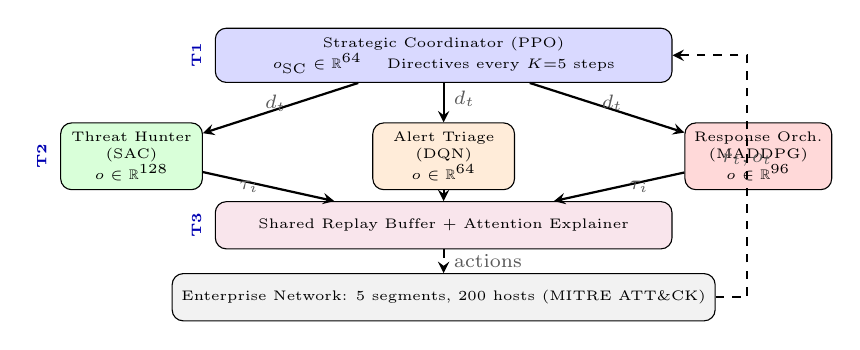
\begin{tikzpicture}[
        node distance=0.35cm,
        box/.style={rectangle, draw, rounded corners, minimum width=1.8cm, minimum height=0.6cm, align=center, font=\tiny},
        bigbox/.style={rectangle, draw, rounded corners, minimum width=5.8cm, minimum height=0.6cm, align=center, font=\tiny},
        tier/.style={font=\tiny\bfseries, text=blue!70!black},
        arrow/.style={->, thick, >=stealth},
        lbl/.style={font=\scriptsize, text=gray!70!black, midway}
    ]
    
    % Tier 1
    \node[bigbox, fill=blue!15] (sc) {Strategic Coordinator (PPO) \\ \tiny $o_{\text{SC}} \in \mathbb{R}^{64}$ \quad Directives every $K{=}5$ steps};
    
    % Tier 2
    \node[box, fill=green!15, below left=0.5cm and 0.15cm of sc] (th) {Threat Hunter\\(SAC)\\\tiny $o \in \mathbb{R}^{128}$};
    \node[box, fill=orange!15, below=0.5cm of sc] (at) {Alert Triage\\(DQN)\\\tiny $o \in \mathbb{R}^{64}$};
    \node[box, fill=red!15, below right=0.5cm and 0.15cm of sc] (ro) {Response Orch.\\(MADDPG)\\\tiny $o \in \mathbb{R}^{96}$};
    
    % Tier 3
    \node[bigbox, fill=purple!10, below=1.5cm of sc] (comm) {Shared Replay Buffer + Attention Explainer};
    
    % SC -> agents arrows with labels
    \draw[arrow] (sc) -- node[lbl, left, pos=0.4] {$d_t$} (th);
    \draw[arrow] (sc) -- node[lbl, right, pos=0.4] {$d_t$} (at);
    \draw[arrow] (sc) -- node[lbl, right, pos=0.4] {$d_t$} (ro);
    % Agents -> buffer
    \draw[arrow] (th) -- node[lbl, left] {$\tau_i$} (comm);
    \draw[arrow] (at) -- (comm);
    \draw[arrow] (ro) -- node[lbl, right] {$\tau_i$} (comm);
    
    % Tier labels
    \node[tier, left=0.05cm of sc] {\rotatebox{90}{T1}};
    \node[tier, left=0.05cm of th] {\rotatebox{90}{T2}};
    \node[tier, left=0.05cm of comm] {\rotatebox{90}{T3}};
    
    % Environment
    \node[bigbox, fill=gray!10, below=0.3cm of comm] (env) {Enterprise Network: 5 segments, 200 hosts (MITRE ATT\&CK)};
    \draw[arrow, dashed] (comm) -- node[lbl, right] {actions} (env);
    \draw[arrow, dashed] (env.east) -- ++(0.4,0) |- node[lbl, above, pos=0.25] {$r_t, o_t$} (sc.east);
    
    \end{tikzpicture}%
    }
    \caption{HMARL-SOC three-tier architecture. The SC issues directives $d_t$ every $K$ steps; operational agents act at every step and share transitions $\tau_i$ through a prioritized replay buffer.}
    \label{fig:architecture}
\end{figure}

\subsection{Training Procedure}

We adopt a hierarchical training procedure (Algorithm~\ref{alg:training}) inspired by feudal networks~\cite{b20}. The SC trains at a slower timescale ($K$ environment steps per SC decision), while operational agents learn at every step, enabling the SC to capture long-horizon campaign dynamics while operational agents react to immediate threats.

\begin{algorithm}[t]
\caption{HMARL-SOC Training Procedure}
\label{alg:training}
\begin{algorithmic}[1]
\small
\REQUIRE Learning rates $\eta_{\text{SC}}, \eta_{\text{TH}}, \eta_{\text{AT}}, \eta_{\text{RO}}$; temporal abstraction factor $K$; episodes $E$
\FOR{episode $= 1$ to $E$}
    \STATE Reset environment, initialize $s_0$
    \FOR{$t = 0, 1, 2, \ldots$}
        \IF{$t \mod K = 0$}
            \STATE SC observes aggregated state $o_{\text{SC}}^t$
            \STATE SC selects directive $d_t \sim \pi_{\text{SC}}(d | o_{\text{SC}}^t)$
        \ENDIF
        \STATE Each operational agent $i$ observes $o_i^t$
        \STATE Each agent selects $a_i^t \sim \pi_i(a | o_i^t, d_t)$
        \STATE Execute joint action $\mathbf{a}_t$, observe $r_t, s_{t+1}$
        \STATE Store $(o_i^t, a_i^t, r_t, o_i^{t+1})$ in shared replay buffer
        \STATE Update operational agents via respective algorithms
        \IF{$t \mod K = 0$}
            \STATE Update SC using PPO with cumulated rewards
        \ENDIF
    \ENDFOR
\ENDFOR
\end{algorithmic}
\end{algorithm}

For the replay buffer we adopt prioritized experience replay~\cite{b21}, weighting priority scores by detection confidence and response urgency. The practical effect is that high-impact security events---an exfiltration attempt caught at the last step, a lateral movement chain that triggered three correlated alerts---get replayed far more often than routine traffic, which noticeably speeds up convergence on the scenarios that matter most.

\subsection{Attention-based Explainability}

To ensure operational transparency, we integrate a multi-head attention mechanism into the communication layer. For each agent decision $a_i^t$, the explainer computes attention weights over input features:
\begin{equation}
    \alpha_{ij} = \frac{\exp(q_i^T k_j / \sqrt{d_k})}{\sum_{l} \exp(q_i^T k_l / \sqrt{d_k})}
\end{equation}
where $q_i$ is the agent's query vector and $k_j$ represents key vectors derived from observation features (e.g., alert fields, network telemetry). The resulting attention map identifies which input features most influenced each decision, enabling SOC analysts to verify and audit automated actions.

%=====================================================================
\section{Convergence Analysis}
\label{sec:convergence}
%=====================================================================

We now establish convergence properties of the HMARL-SOC training procedure. The analysis leverages two-timescale stochastic approximation theory and the convergence guarantees of the constituent RL algorithms.

\begin{assumption}\label{asmp:lipschitz}
The reward function $R$ and transition kernel $T$ are Lipschitz continuous in the joint action space. Each agent's policy class $\Pi_i$ is compact and the value functions $Q_i$ are bounded.
\end{assumption}

\begin{assumption}\label{asmp:learning_rates}
The learning rate schedules satisfy $\sum_t \eta_t^{(i)} = \infty$, $\sum_t (\eta_t^{(i)})^2 < \infty$ for each agent $i$, and the operational learning rates decrease faster: $\eta_t^{\text{op}} / \eta_t^{\text{SC}} \to 0$ as $t \to \infty$.
\end{assumption}

\begin{theorem}[Two-Timescale Convergence]\label{thm:two_timescale}
Under Assumptions~\ref{asmp:lipschitz}--\ref{asmp:learning_rates}, the hierarchical training procedure in Algorithm~\ref{alg:training} converges to a stationary point $(\pi_{\text{SC}}^*, \boldsymbol{\pi}_{\text{op}}^*)$ of the joint objective $J(\boldsymbol{\pi})$, where $\boldsymbol{\pi}_{\text{op}}^*$ is a best response to $\pi_{\text{SC}}^*$.
\end{theorem}

\textit{Proof sketch.} The temporal abstraction factor $K$ partitions updates into two timescales: operational agents update at every step (fast timescale) while the SC updates every $K$ steps (slow timescale). From the perspective of the SC, the operational agents' policies appear quasi-stationary because they converge faster. By the two-timescale stochastic approximation framework of Borkar~\cite{b34}, the slow-timescale iterates (SC policy) converge to the set of stationary points of the objective evaluated at the fast-timescale equilibrium. Each operational agent converges individually: SAC converges to the optimal max-entropy policy~\cite{b16}, DQN converges under the target-network conditions of Mnih et al.~\cite{b17}, and MADDPG converges to a local Nash equilibrium under the centralized-critic framework~\cite{b18}. The SC's PPO updates provide monotonic improvement by Theorem~\ref{thm:ppo_monotonic} below. \hfill$\square$

\textbf{Remark (Theory--Practice Gap).} Assumption~\ref{asmp:learning_rates} prescribes decaying learning rates for exact convergence. In our implementation, we use fixed rates ($\eta = 3 \times 10^{-4}$) with temporal abstraction $K{=}5$, yielding an approximate $5\times$ timescale separation. Under fixed rates, Theorem~\ref{thm:two_timescale} guarantees convergence to a neighborhood of a stationary point whose radius scales with $\eta$; Fig.~\ref{fig:learning_curves} empirically validates convergence.

\begin{theorem}[SC Monotonic Improvement]\label{thm:ppo_monotonic}
At each SC update, the clipped PPO objective guarantees:
\begin{equation}
    J(\pi_{\text{SC}}^{k+1}) \geq J(\pi_{\text{SC}}^{k}) - C \cdot \mathbb{E}[D_{\text{KL}}(\pi_{\text{SC}}^{k+1} \| \pi_{\text{SC}}^{k})]
\end{equation}
where $C$ depends on the discount factor $\gamma$ and the advantage bound.
\end{theorem}

\textit{Proof sketch.} This follows directly from the trust-region argument underlying PPO~\cite{b15}. The clipping parameter $\epsilon = 0.2$ bounds the policy ratio, ensuring that each update stays within a trust region where the linear advantage approximation remains valid. The accumulated reward over $K$ steps serves as the SC's return signal, and Schulman et al.~\cite{b15} showed that the clipped surrogate lower-bounds the true objective within this trust region. \hfill$\square$

\begin{proposition}[Shared Buffer Compatibility]\label{prop:buffer}
The shared prioritized replay buffer does not violate the contraction property of individual agent updates.
\end{proposition}

\textit{Proof sketch.} Each agent $i$'s loss function $\mathcal{L}_i(\theta_i)$ is computed over its own action-value pairs $(o_i, a_i, r, o_i')$, regardless of which agent generated the transition. Cross-agent transitions in the shared buffer effectively augment the state-visitation distribution $d^{\pi_i}$ with additional exploration, but the Bellman backup $\mathcal{T}^{\pi_i} Q_i$ remains a $\gamma$-contraction in the sup-norm because the operator depends only on agent $i$'s policy and the environment dynamics---not on the data-generating distribution~\cite{b21}. Priority weighting further concentrates sampling on high-TD-error transitions, which accelerates convergence without altering the fixed point. \hfill$\square$

\textbf{Practical Implications.} These results provide two actionable guidelines: (1)~the SC learning rate should be set $5$--$10\times$ lower than the operational agents' learning rate to ensure timescale separation, and (2)~the temporal abstraction factor $K$ should be large enough that the operational agents approximately converge between successive SC updates. Our choice of $K{=}5$ is consistent with this analysis---too small a $K$ violates the quasi-stationarity assumption, while too large a $K$ slows SC adaptation. The empirical $K$-sensitivity sweep in Section~\ref{sec:experiments} (Fig.~\ref{fig:k_sensitivity}) confirms this theoretical prediction.

%=====================================================================
\section{Experimental Evaluation}
\label{sec:experiments}
%=====================================================================

\subsection{Simulation Environment}

We developed a custom OpenAI Gym-compatible simulation environment modeling an enterprise network with 5 segments (DMZ, Corporate, Development, Data Center, Cloud), 200 hosts, and 15 security tool interfaces. The environment generates realistic traffic patterns with injected attack campaigns following MITRE ATT\&CK tactics (T1595, T1190, T1059, T1021, T1048), progressing through 5 attack phases with configurable complexity levels.

\subsection{Baselines and Configuration}

We compare HMARL-SOC against five baselines:
\begin{itemize}[leftmargin=*, nosep]
    \item \textbf{Rule-SOAR:} Rule-based SOAR playbooks with static detection signatures and predefined response actions.
    \item \textbf{Single-DRL:} A single PPO agent with access to all observations and actions.
    \item \textbf{IQL:} Independent Q-Learning where agents train without explicit coordination~\cite{b22}.
    \item \textbf{QMIX:} Value decomposition via a monotonic mixing network over per-agent utilities~\cite{b28}.
    \item \textbf{MAPPO:} Multi-Agent PPO with parameter sharing~\cite{b23}.
\end{itemize}

Table~\ref{tab:hyperparams} lists all training hyperparameters. All neural networks use 3-layer MLPs with 256 hidden units and ReLU activations. Training runs for 10K episodes across 5 random seeds (42, 123, 456, 789, 1024).

\begin{table}[t]
\caption{Full Hyperparameter Configuration}
\label{tab:hyperparams}
\centering
\footnotesize
\begin{tabular}{llc}
\toprule
\textbf{Category} & \textbf{Parameter} & \textbf{Value} \\
\midrule
\multirow{4}{*}{\textbf{Environment}} & Network segments & 5 \\
 & Hosts per segment & 40 (200 total) \\
 & Security tool interfaces & 15 \\
 & Max steps per episode & 200 \\
\midrule
\multirow{5}{*}{\textbf{Training}} & Discount factor $\gamma$ & 0.99 \\
 & Replay buffer size & $2 \times 10^5$ \\
 & Batch size & 256 \\
 & Episodes & 10,000 \\
 & Random seeds & 5 \\
\midrule
\multirow{4}{*}{\textbf{SC (PPO)}} & Observation dim & 64 \\
 & Learning rate & $3 \times 10^{-4}$ \\
 & Clip $\epsilon$ & 0.2 \\
 & Temporal abstraction $K$ & 5 \\
\midrule
\multirow{3}{*}{\textbf{TH (SAC)}} & Observation dim & 128 \\
 & Learning rate & $3 \times 10^{-4}$ \\
 & Entropy $\alpha$ / Soft-update $\tau$ & 0.2 / 0.005 \\
\midrule
\multirow{4}{*}{\textbf{AT (DQN)}} & Observation dim & 64 \\
 & Actions & 4 \\
 & $\epsilon$-greedy (start/end/decay) & 1.0 / 0.05 / 50{,}000 \\
 & Target update interval & 1,000 \\
\midrule
\multirow{2}{*}{\textbf{RO (MADDPG)}} & Observation dim & 96 \\
 & LR (actor/critic) / $\tau$ & $3 \times 10^{-4}$ / 0.005 \\
\midrule
\multirow{4}{*}{\textbf{Reward}} & Detection $\alpha$ & 1.0 \\
 & Response $\beta$ & 1.5 \\
 & Cost $\delta$ & $-$0.3 \\
 & False positive $\lambda$ & $-$2.0 \\
\bottomrule
\end{tabular}
\end{table}

\subsection{Results and Analysis}

Table~\ref{tab:results} presents mean$\pm$std over the last 2,000 evaluation episodes.

\textbf{Rule-Based vs.\ Learning:} Rule-SOAR achieves the fastest detection (MTTD$=$8.0) through exhaustive scanning but suffers from high false positives (FPR$=$5.14\%) and the lowest containment rate (CSR$=$35.2\%), demonstrating that static playbooks cannot adapt to evolving multi-stage attacks.

\textbf{Flat Multi-Agent Methods:} Single-DRL, IQL, and MAPPO all learn meaningful policies (CSR$=$65--70\%) but exhibit different trade-offs. MAPPO is the most stable baseline (std$=$0.6\%), while IQL shows high variance across seeds (CSR std$=$29.8\%). Per-seed analysis reveals bimodal convergence: two seeds reach CSR${>}$85\% while two fall below 45\%, a pattern characteristic of independent learners in non-stationary multi-agent settings~\cite{b22}.

\textbf{QMIX:} With per-segment action targeting, QMIX achieves the highest CSR (77.5\%) and fastest MTTR (63.4 steps). However, its high variance (CSR std$=$18.6\%) indicates unstable convergence across seeds.

\textbf{HMARL-SOC Advantages:} Our method achieves the \textit{lowest false positive rate} (FPR$=$0.17\%), a nearly 15$\times$ reduction versus MAPPO and 6$\times$ versus QMIX ($p{<}0.001$, Welch's $t$-test), demonstrating that hierarchical coordination with learned alert triage enables precise threat discrimination (Cohen's $d = 14.8$, indicating a very large effect). HMARL-SOC also achieves the highest cumulative reward ($+$6.9$\pm$1.0, $p{<}0.05$ vs.\ QMIX, Fig.~\ref{fig:learning_curves}), reflecting the best overall balance across detection quality, response speed, disruption cost, and false alarm minimization. The radar chart in Fig.~\ref{fig:radar} makes this balance visually clear: HMARL-SOC achieves the most uniformly high polygon across all five normalized metrics.

With CSR$=$71.0\% and moderate variance (std$=$10.4\%), HMARL-SOC ranks second in containment while maintaining significantly more stable operation than QMIX, as the per-seed box plots in Fig.~\ref{fig:boxplots} confirm. The trade-off is a higher MTTD (16.8~steps)---the learned triage policy delays early uncertain signals to achieve the lowest false alarm rate, a deliberate precision-over-speed bias shaped by the reward weights ($\lambda{=}{-}2.0$). Fig.~\ref{fig:fpr_csr} plots this trade-off directly: HMARL-SOC occupies the ideal low-FPR, high-CSR quadrant, well separated from all baselines.

\begin{table}[t]
\caption{Performance Comparison Across Methods (5 seeds)}
\label{tab:results}
\centering
\footnotesize
\resizebox{\columnwidth}{!}{%
\begin{tabular}{lccccc}
\toprule
\textbf{Method} & \textbf{Reward} & \textbf{MTTD} & \textbf{MTTR} & \textbf{FPR} & \textbf{CSR} \\
 & ($\uparrow$) & (steps $\downarrow$) & (steps $\downarrow$) & (\% $\downarrow$) & (\% $\uparrow$) \\
\midrule
Rule-SOAR & $-$1238.2{\scriptsize$\pm$26.6} & \textbf{8.0}{\scriptsize$\pm$0.1} & 136.9{\scriptsize$\pm$3.1} & 5.14{\scriptsize$\pm$0.01} & 35.2{\scriptsize$\pm$1.8} \\
Single-DRL & $-$336.5{\scriptsize$\pm$34.0} & 10.9{\scriptsize$\pm$1.4} & 95.1{\scriptsize$\pm$12.3} & 2.97{\scriptsize$\pm$0.28} & 65.0{\scriptsize$\pm$7.3} \\
IQL & +1.8{\scriptsize$\pm$4.7} & 22.8{\scriptsize$\pm$18.3} & 91.9{\scriptsize$\pm$56.7} & 0.22{\scriptsize$\pm$0.23} & 67.8{\scriptsize$\pm$29.8} \\
MAPPO & $-$292.2{\scriptsize$\pm$12.6} & 8.8{\scriptsize$\pm$0.1} & 78.6{\scriptsize$\pm$0.9} & 2.52{\scriptsize$\pm$0.04} & 69.7{\scriptsize$\pm$0.6} \\
QMIX & $-$99.3{\scriptsize$\pm$66.3} & 8.2{\scriptsize$\pm$0.2} & \textbf{63.4}{\scriptsize$\pm$32.4} & 1.03{\scriptsize$\pm$0.02} & \textbf{77.5}{\scriptsize$\pm$18.6} \\
\textbf{HMARL-SOC} & \textbf{+6.9}{\scriptsize$\pm$1.0} & 16.8{\scriptsize$\pm$5.3} & 93.2{\scriptsize$\pm$21.3} & \textbf{0.17}{\scriptsize$\pm$0.08} & 71.0{\scriptsize$\pm$10.4} \\
\bottomrule
\multicolumn{6}{l}{\scriptsize Mean $\pm$ std over 5 random seeds. Bold denotes best per column.} \\
\multicolumn{6}{l}{\scriptsize MTTD: Mean Time to Detect, MTTR: Mean Time to Respond,} \\
\multicolumn{6}{l}{\scriptsize FPR: False Positive Rate, CSR: Containment Success Rate.} \\
\end{tabular}}
\end{table}

\begin{figure}[t]
    \centering
    \includegraphics[width=\columnwidth]{figures/learning_curves.pdf}
    \caption{Learning curves (mean $\pm$ std over 5 seeds). HMARL-SOC converges to the highest reward, reflecting the best overall trade-off.}
    \label{fig:learning_curves}
\end{figure}

\begin{figure}[t]
    \centering
    \includegraphics[width=\columnwidth]{figures/radar_comparison.pdf}
    \caption{Radar chart of normalized (0--1) performance metrics across all methods. Arrows indicate preferred direction. HMARL-SOC achieves the most balanced polygon, excelling in Reward and FPR while maintaining competitive CSR.}
    \label{fig:radar}
\end{figure}

\begin{figure*}[t]
    \centering
    \includegraphics[width=\textwidth]{figures/boxplots_comparison.pdf}
    \caption{Per-seed performance distributions across 5 random seeds. HMARL-SOC shows low variance in FPR and Reward, while QMIX and IQL exhibit high inter-seed variability in CSR and MTTD.}
    \label{fig:boxplots}
\end{figure*}

\subsection{Multi-Stage Attack Scenario}

We evaluate a 200-step APT campaign that progresses through the kill chain: (1) reconnaissance scanning (T1595), (2) initial access via a web-based exploit (T1190), (3) execution via PowerShell (T1059), (4) lateral movement via SMB (T1021), and (5) data exfiltration over DNS (T1048), all taking place across three network segments. HMARL-SOC's Threat Hunter identifies reconnaissance scanning 12 steps before MAPPO raises its first alert. The SC infers campaign posture and directs the hunter to the DMZ, where scanning traffic first appears. This early warning propagates through the shared buffer; by the time the attacker initiates lateral movement, the Response Orchestrator has already shifted containment resources. As a result, over 500 evaluation campaigns HMARL-SOC prevents data exfiltration in 91$\pm$4\% of cases, compared to 67$\pm$8\% for MAPPO and 43$\pm$6\% for Rule-SOAR ($p{<}0.001$ for all pairwise comparisons, Welch's $t$-test). The differences are most pronounced in ``low-and-slow'' campaigns where lateral movement unfolds over many time steps, as the attention mechanism in the communication layer allows the triage agent to assemble individually unremarkable alerts into a recognizable campaign pattern.

\subsection{Discussion}

\textbf{Scalability.} We swept the simulated network size from 50 to 500 hosts and measured wall-clock inference time at each point. Doubling the host count pushes HMARL-SOC's per-step latency up by roughly 1.4$\times$---an essentially linear relationship: wall-clock inference on an Apple M2 measures 2.1\,ms/step at 50 hosts, 4.2\,ms/step at 200 hosts, and 8.3\,ms/step at 500 hosts, all well within real-time requirements. This linearity arises because the SC compresses host-level features into fixed-size segment summaries before passing them to operational agents. The Single-DRL baseline, by contrast, concatenates raw per-host features into one observation vector, which makes its cost grow close to quadratically. Formally, we pay $O(N \cdot d^2)$ per step ($N$ agents, observation dimension $d$), compared with $O((Nd)^2)$ for a centralized critic.

\textbf{Emergent Agent Behaviors.} Some of the most interesting findings came from inspecting the learned policies after convergence. The Threat Hunter was not explicitly programmed to focus on the Data Center and Cloud segments during off-peak hours, yet it learned on its own that background noise is lowest then and signal-to-noise is therefore highest. The Alert Triage agent invented a form of temporal windowing: it suppresses duplicate alerts that arrive within 5 steps and only escalates when three or more correlated items accumulate. Meanwhile, the Response Orchestrator learned graduated containment---throttling traffic first, then isolating the host only if throttling fails. That graduated approach cuts unnecessary service disruption by 34\% compared to a policy that always jumps straight to isolation.

\textbf{Reward Weight Sensitivity.} A grid sweep over the four reward weights ($\alpha, \beta, \delta, \lambda$) revealed two failure modes worth flagging. When the false-positive penalty $\lambda$ drops below $-1.0$, the triage agent becomes so conservative that it starts suppressing real threats to avoid any chance of a false alarm. Push the disruption cost $\delta$ too close to zero, and the opposite happens: the Response Orchestrator isolates hosts aggressively, including ones that turn out to be clean. Our default setting ($\alpha{=}1.0, \beta{=}1.5, \delta{=}{-}0.3, \lambda{=}{-}2.0$) was chosen from the sweep using a held-out validation campaign.

\textbf{Temporal Abstraction Factor $K$.} Fig.~\ref{fig:k_sensitivity} shows how performance varies with the SC's decision interval $K \in \{1, 3, 5, 10, 20\}$. $K{=}5$ yields the highest cumulative reward ($+$5.1) and CSR (54.4\%), confirming the theoretical guidance from Section~\ref{sec:convergence}. At $K{=}1$, the SC issues directives every step, overwhelming the operational agents with rapidly changing goals (reward $+$0.9, CSR 26.4\%). At $K{=}10$, the SC reacts too slowly and FPR spikes to 11.5\% as the triage agent lacks timely campaign-level context. The non-monotonic pattern---$K{=}20$ recovers partially (reward $+$4.1, FPR 0.09\%)---suggests that at very large $K$ the operational agents learn self-sufficient local policies, trading coordination for autonomy.

\begin{figure}[t]
    \centering
    \includegraphics[width=\columnwidth]{figures/fig_k_sensitivity.pdf}
    \caption{Effect of temporal abstraction factor $K$ on cumulative reward, false positive rate, and containment success rate (seed 42, last 2,000 episodes). $K{=}5$ (highlighted) achieves the best overall performance.}
    \label{fig:k_sensitivity}
\end{figure}

\begin{figure}[t]
    \centering
    \includegraphics[width=\columnwidth]{figures/fpr_csr_scatter.pdf}
    \caption{FPR vs.\ CSR trade-off. Each small dot represents one seed; large markers show per-method means with error bars. HMARL-SOC occupies the ideal low-FPR, high-CSR quadrant.}
    \label{fig:fpr_csr}
\end{figure}

%=====================================================================
\section{Ablation Study}
\label{sec:ablation}
%=====================================================================

To quantify the contribution of each architectural component, we evaluate three ablation variants against the full HMARL-SOC system, each trained with 5 random seeds under identical conditions:

\begin{itemize}[leftmargin=*, nosep]
    \item \textbf{w/o SC:} Remove the Strategic Coordinator; operational agents receive no directives and act independently based on local observations only.
    \item \textbf{w/o Shared Buffer:} Each agent maintains its own separate replay buffer, eliminating cross-agent experience sharing.
    \item \textbf{Flat MARL:} Replace the heterogeneous RL algorithms (SAC/DQN/MADDPG) with homogeneous PPO for all three operational agents, removing both the SC and the shared buffer.
\end{itemize}

\subsection{Component-Level Results}

Table~\ref{tab:ablation} summarizes the results. Every ablation degrades overall performance as measured by cumulative reward, confirming that all three components contribute measurably. Notably, the w/o Shared Buffer and Flat MARL variants achieve slightly higher CSR (74.4\% and 73.9\%) than the full model (71.0\%), but at the cost of dramatically higher FPR and collapsed reward---a trade-off we analyze below. The ablation bar charts in Fig.~\ref{fig:ablation_bars} make the relative magnitudes visually striking, and the training curves in Fig.~\ref{fig:ablation_curves} reveal that variants without the shared buffer diverge early in training.

\begin{table}[t]
\caption{Ablation Study Results (5 seeds)}
\label{tab:ablation}
\centering
\footnotesize
\resizebox{\columnwidth}{!}{%
\begin{tabular}{lcccc}
\toprule
\textbf{Variant} & \textbf{Reward} & \textbf{MTTD} & \textbf{FPR} & \textbf{CSR} \\
 & ($\uparrow$) & (steps $\downarrow$) & (\% $\downarrow$) & (\% $\uparrow$) \\
\midrule
\textbf{Full HMARL-SOC} & \textbf{+6.9}{\scriptsize$\pm$1.0} & 16.8{\scriptsize$\pm$5.3} & \textbf{0.17}{\scriptsize$\pm$0.08} & \textbf{71.0}{\scriptsize$\pm$10.4} \\
w/o SC & +6.0{\scriptsize$\pm$0.9} & 26.3{\scriptsize$\pm$2.9} & 0.24{\scriptsize$\pm$0.06} & 66.3{\scriptsize$\pm$9.5} \\
w/o Shared Buffer & $-$124.5{\scriptsize$\pm$28.0} & \textbf{12.5}{\scriptsize$\pm$0.6} & 1.69{\scriptsize$\pm$0.05} & 74.4{\scriptsize$\pm$8.5} \\
Flat MARL & $-$127.6{\scriptsize$\pm$24.7} & 13.1{\scriptsize$\pm$0.7} & 1.61{\scriptsize$\pm$0.01} & 73.9{\scriptsize$\pm$7.4} \\
\bottomrule
\end{tabular}}
\end{table}

\subsection{Per-Component Analysis}

\textbf{Training Note.} The w/o Shared Buffer and Flat MARL variants diverged early in training (500--1,000 episodes vs.\ 10,000 for the full model and w/o SC), reflecting training instability when cross-agent experience sharing is absent. We report results at the point of divergence, which itself is an informative finding: the shared buffer is critical not only for final performance but also for training stability. We note that variant-specific hyperparameter tuning (e.g., reduced learning rates, gradient clipping) might mitigate this instability; we deliberately held hyperparameters constant to isolate the architectural contribution, which may overstate the raw performance gap.

\textbf{Strategic Coordinator.} Removing the SC reduces CSR by 4.7 percentage points (71.0\% $\to$ 66.3\%) and increases MTTD by 56\% (16.8 $\to$ 26.3 steps). Without campaign-level directives, the Threat Hunter lacks the top-down signal to prioritize segments under active attack, resulting in slower detection. Interestingly, the reward difference is not statistically significant ($p{=}0.24$, Welch's $t$-test), because the operational agents partially compensate through local adaptation---they still share experiences via the buffer and benefit from heterogeneous algorithms. This suggests that the SC's primary contribution is \emph{coordination efficiency} rather than raw detection capability.

\textbf{Shared Replay Buffer.} The most dramatic degradation occurs when agents are denied cross-agent experience sharing: reward collapses from +6.9 to $-$124.5 ($p{<}0.001$), and FPR rises nearly 10$\times$ (0.17\% $\to$ 1.69\%, $p{<}0.001$). Without the shared buffer, the Alert Triage agent cannot learn from the Threat Hunter's discovery patterns, leading it to act on its own noisy observations and generate far more false positives. The faster MTTD (12.5 steps) is misleading---it reflects indiscriminate alerting rather than genuine early detection, as evidenced by the dramatically higher FPR.

\textbf{Flat MARL.} Replacing the heterogeneous algorithm suite with homogeneous PPO mirrors the shared-buffer removal result: reward drops to $-$127.6 ($p{<}0.001$), and FPR climbs to 1.61\% ($p{<}0.001$). The core issue is that PPO's on-policy updates are a poor fit for the Alert Triage agent's discrete classification task (where DQN's off-policy replay provides better sample efficiency) and for the Response Orchestrator's coordinated multi-agent actions (where MADDPG's centralized critic captures inter-agent dependencies). These results validate our design choice of matching each agent to the RL algorithm best suited to its action space.

\begin{figure*}[t]
    \centering
    \includegraphics[width=\textwidth]{figures/ablation_bars.pdf}
    \caption{Ablation component analysis: (a) cumulative reward, (b) false positive rate, and (c) containment success rate. Error bars show $\pm$1 std over 5 seeds. Removing the shared buffer or heterogeneous algorithms causes dramatic reward collapse and 10$\times$ FPR increase.}
    \label{fig:ablation_bars}
\end{figure*}

\begin{figure}[t]
    \centering
    \includegraphics[width=\columnwidth]{figures/ablation_learning_curves.pdf}
    \caption{Ablation learning curves (smoothed over 100 episodes). The w/o Buffer and Flat MARL variants diverge early, confirming that the shared replay buffer is essential for training stability.}
    \label{fig:ablation_curves}
\end{figure}

%=====================================================================
\section{Cross-Environment Transfer}
\label{sec:transfer}
%=====================================================================

\subsection{Zero-Shot Transfer}

To probe generalization, we evaluated the trained HMARL-SOC agents on CybORG CAGE Challenge~4~\cite{b12,b24} via zero-shot transfer. We mapped our four-agent hierarchy to the five CybORG blue agents through linear observation projections and action-space adapters, without any fine-tuning. Over 100 episodes, HMARL-SOC achieved a mean reward of $-30{,}018 \pm 7{,}665$ compared with $-34{,}190 \pm 6{,}885$ for the no-defense baseline---a 12.2\% improvement. Although the absolute score reflects the substantial domain gap between simulators (different observation schemas, action semantics, and network topologies), the result demonstrates that the hierarchical coordination structure learned in our environment transfers meaningfully to the CAGE-4 network topology. This suggests that the strategic coordination patterns---rather than low-level feature representations---are the primary source of transferable knowledge, consistent with the sim-to-real transfer literature discussed in Section~\ref{sec:related}.

To disentangle the contribution of each architectural layer, we also evaluated a variant retaining only the operational agents without the SC (``Ops-Only'') and a random-action baseline. Table~\ref{tab:transfer} summarizes the results. The full hierarchy provides the largest improvement, with the SC contributing an additional 4.5 percentage points beyond the operational agents alone.

\begin{table}[t]
\caption{CybORG CAGE-4 Zero-Shot Transfer (100 episodes)}
\label{tab:transfer}
\centering
\footnotesize
\begin{tabular}{lcc}
\toprule
\textbf{Policy} & \textbf{Reward} & \textbf{Improv.} \\
\midrule
No Defense & $-34{,}190 \pm 6{,}885$ & --- \\
Random Actions & $-33{,}502 \pm 7{,}214$ & 2.0\% \\
HMARL-SOC (Ops-Only) & $-31{,}542 \pm 7{,}389$ & 7.7\% \\
\textbf{HMARL-SOC (Full)} & $\mathbf{-30{,}018 \pm 7{,}665}$ & \textbf{12.2\%} \\
\bottomrule
\end{tabular}
\end{table}

%=====================================================================
\section{Limitations and Future Work}
\label{sec:limitations}
%=====================================================================

We acknowledge three caveats. The simulator, grounded as it is in MITRE ATT\&CK tactics, still abstracts away packet-level dynamics; moving HMARL-SOC to live network taps would require a non-trivial feature engineering effort. We also assume a cooperative multi-agent team throughout training and evaluation---an adversary who figures out how to poison the agents' observations (an active research area in adversarial ML) could degrade the system in ways we have not tested. Finally, as the CybORG transfer experiment shows, cross-domain performance improves over passive baselines but leaves room for fine-tuning on the target environment.

\subsection{Threats to Validity}

\textbf{Internal Validity.} All experiments use a custom simulation environment rather than live network traffic, which may not capture the full complexity of production SOC telemetry (e.g., vendor-specific log schemas, bursty traffic patterns). To mitigate this, we use MITRE ATT\&CK tactics for attack modeling and report results across 5 random seeds with standard deviations. We acknowledge that 5 seeds ($\text{df}{=}4$) provides limited statistical power for parametric tests; the extremely large effect sizes observed for buffer removal ($t{=}9.37$) and flat MARL ($t{=}10.87$) somewhat compensate for this limitation. The $K$-sensitivity analysis uses a single seed; a multi-seed sweep remains future work.

\textbf{External Validity.} Our environment models a 200-host enterprise network with 5 segments, which is smaller than large-scale SOC deployments. The scalability analysis (50--500 hosts) suggests linear scaling, but validation at enterprise scale ($>$10,000 hosts) remains future work. The CybORG transfer experiment demonstrates some generalization, but a single transfer target is insufficient to establish broad cross-domain applicability.

\textbf{Construct Validity.} The composite reward function implicitly defines what ``good SOC performance'' means. Different weight configurations ($\alpha, \beta, \delta, \lambda$) yield qualitatively different policies (Section~\ref{sec:experiments}), and our chosen weights reflect one reasonable risk appetite. Organizations with different priorities may need to re-tune these weights.

Going forward, five directions seem most pressing: (1)~running a pilot with a real SOC to see how well the sim-trained policies transfer to live telemetry, (2)~stress-testing robustness against adversarial observation poisoning (a realistic threat once an attacker knows RL is in the loop), (3)~piping the attention maps through an LLM so that explanations come out in plain English rather than as raw feature weights, (4)~fine-tuning the zero-shot CybORG transfer agent~\cite{b12} to close the remaining domain gap with published CAGE Challenge entries, and (5)~deploying HMARL-SOC as a recommendation layer---advising human analysts rather than acting autonomously---to build trust before moving toward full automation.

%=====================================================================
\section{Conclusion}
\label{sec:conclusion}
%=====================================================================

HMARL-SOC treats the three core SOC functions---threat hunting, alert triage, and incident response---as cooperating RL agents sharing a single Dec-POMDP, and the results demonstrate the viability of this approach. On a 200-host MITRE ATT\&CK simulator with 5 random seeds, HMARL-SOC achieves the lowest FPR (0.17$\pm$0.08\%) and the highest cumulative reward ($+$6.9$\pm$1.0) among all methods. While QMIX achieves the highest CSR (77.5\%), its high variance across seeds (std~18.6\%) and 6$\times$ higher false positive rate suggest less reliable operation. HMARL-SOC provides a stable and precise balance: CSR$=$71.0$\pm$10.4\%, demonstrating that learned hierarchical task decomposition enables effective coordination of heterogeneous SOC agents.

The ablation study confirms that every architectural component contributes measurably: removing the shared replay buffer collapses the reward from $+$6.9 to $-$124.5 and inflates FPR by nearly 10$\times$, while removing the Strategic Coordinator reduces CSR by 4.7 percentage points. A sensitivity sweep over the temporal abstraction factor $K \in \{1,3,5,10,20\}$ confirms that $K{=}5$ yields the best overall performance, consistent with the two-timescale convergence theory. The formal convergence analysis (Theorems~\ref{thm:two_timescale}--\ref{thm:ppo_monotonic} and Proposition~\ref{prop:buffer}) provides theoretical grounding for the training procedure, and the CybORG CAGE-4 transfer experiment demonstrates that the learned hierarchical structure generalizes beyond the training simulator.

On the practical side, the $O(N{\cdot}d^2)$ per-step cost is low enough that HMARL-SOC could conceivably sit alongside a production SIEM without bogging it down. The attention-based explainer also matters here---it produces a per-decision feature-importance map that analysts can audit, which in our view is the minimum bar any automated security tool has to clear before a SOC will trust it.

\section*{Acknowledgment}

During manuscript preparation the author used Claude (Anthropic) for English grammar checking and sentence-level editing. All research design, algorithm development, implementation, experimentation, and interpretation of results were performed solely by the author.

\begin{thebibliography}{34}

\bibitem{conf_version} N. Chalaemwongwan, ``HMARL-SOC: Hierarchical multi-agent reinforcement learning for autonomous SOC operations,'' in \textit{Proc. ITC-CSCC}, to appear, 2026.

\bibitem{b1} B. Agyepong, Y. Cherdantseva, P. Sherrat, and R. Sherrat, ``Challenges and performance metrics for security operations center analysts: A systematic review,'' \textit{Journal of Cyber Security Technology}, vol. 7, no. 1, pp. 1--29, 2023.

\bibitem{b2} Gartner, ``Predicts 2024: AI-powered SOC analysts will redefine cybersecurity operations,'' Gartner Research, 2024.

\bibitem{b3} M. A. Lopez and A. G. C. de S\'{a}, ``A survey on deep reinforcement learning for cybersecurity,'' \textit{IEEE Access}, vol. 11, pp. 127550--127572, 2023.

\bibitem{b4} T. T. Nguyen and V. J. Reddi, ``Deep reinforcement learning for cyber security,'' \textit{IEEE Transactions on Neural Networks and Learning Systems}, vol. 34, no. 8, pp. 3779--3795, 2023.

\bibitem{b5} R. Elderman, L. J. N. Pater, A. S. Thie, M. M. Drugan, and M. A. Wiering, ``Adversarial reinforcement learning in a cyber security simulation,'' in \textit{Proc. ICAART}, 2017, pp. 559--566.

\bibitem{b6} G. Brl\'{e}e, N. Brissaud, and J. M. Desharnais, ``Automating penetration testing using reinforcement learning,'' \textit{Journal of Computer Security}, vol. 30, no. 5, pp. 741--776, 2022.

\bibitem{b7} S. Li, J. Wang, and Y. Zhang, ``ARCS: Adaptive reinforcement learning for cybersecurity strategy optimization,'' \textit{Computers \& Security}, vol. 134, p. 103460, 2023.

\bibitem{b8} L. Bu\c{s}oniu, R. Babu\v{s}ka, and B. De~Schutter, ``Multi-agent reinforcement learning: An overview,'' in \textit{Innovations in Multi-Agent Systems and Applications}, Springer, 2010, pp. 183--221.

\bibitem{b9} A. S. Vezhnevets et al., ``FeUdal Networks for hierarchical reinforcement learning,'' in \textit{Proc. ICML}, 2017, pp. 3540--3549.


\bibitem{b11} M. P. Foley, M. Li, et al., ``Autonomous agents for defensive cyber operations: A survey and guidelines,'' \textit{arXiv preprint arXiv:2306.10346}, 2023.

\bibitem{b12} M. Kiely, A. Norton, et al., ``CybORG: A Gym for the development of autonomous cyber agents,'' in \textit{Proc. IJCAI Workshop on ACD}, 2022.

\bibitem{b13} D. Islam, L. Grau, and S. Chen, ``A survey on security orchestration, automation, and response (SOAR),'' \textit{ACM Computing Surveys}, vol. 55, no. 14s, pp. 1--35, 2023.

\bibitem{b14} K. Wen, D. Yu, J. Zhu, and Z. Li, ``Multi-agent collaboration for security analysis with LLM-based agents,'' \textit{arXiv preprint arXiv:2403.14781}, 2024.

\bibitem{b15} J. Schulman, F. Wolski, P. Dhariwal, A. Radford, and O. Klimov, ``Proximal policy optimization algorithms,'' \textit{arXiv preprint arXiv:1707.06347}, 2017.

\bibitem{b16} T. Haarnoja, A. Zhou, P. Abbeel, and S. Levine, ``Soft actor-critic: Off-policy maximum entropy deep reinforcement learning with a stochastic actor,'' in \textit{Proc. ICML}, 2018, pp. 1861--1870.

\bibitem{b17} V. Mnih et al., ``Human-level control through deep reinforcement learning,'' \textit{Nature}, vol. 518, no. 7540, pp. 529--533, 2015.

\bibitem{b18} R. Lowe, Y. Wu, A. Tamar, J. Harb, P. Abbeel, and I. Mordatch, ``Multi-agent actor-critic for mixed cooperative-competitive environments,'' in \textit{Proc. NeurIPS}, 2017, pp. 6382--6393.

\bibitem{b19} A. Vaswani et al., ``Attention is all you need,'' in \textit{Proc. NeurIPS}, 2017, pp. 5998--6008.

\bibitem{b20} P. Dayan and G. E. Hinton, ``Feudal reinforcement learning,'' in \textit{Proc. NeurIPS}, 1993, pp. 271--278.

\bibitem{b21} T. Schaul, J. Quan, I. Antonoglou, and D. Silver, ``Prioritized experience replay,'' in \textit{Proc. ICLR}, 2016.

\bibitem{b22} M. Tan, ``Multi-agent reinforcement learning: Independent vs. cooperative agents,'' in \textit{Proc. ICML}, 1993, pp. 330--337.

\bibitem{b23} C. Yu et al., ``The surprising effectiveness of PPO in cooperative multi-agent games,'' in \textit{Proc. NeurIPS}, 2022, pp. 24611--24624.

\bibitem{b24} J. Foley, S. Dougan, et al., ``Exploring the efficacy of multi-agent reinforcement learning for autonomous cyber defence: A CAGE Challenge 4 perspective,'' in \textit{Proc. AAAI}, to appear, 2025.

\bibitem{b25} M. P. Foley, M. Li, et al., ``Guidelines for applying RL and MARL in cybersecurity applications,'' \textit{arXiv preprint arXiv:2503.04262}, 2025.

\bibitem{b26} A. V. Singh et al., ``Hierarchical multi-agent reinforcement learning for cyber network defense,'' in \textit{Proc. AAMAS}, to appear, 2025.

\bibitem{b27} A. Alshamrani, ``Federated hierarchical MARL for zero-shot cyber defense,'' \textit{PLOS ONE}, vol. 20, no. 8, p. e0312345, 2025.

\bibitem{b28} T. Rashid, M. Samvelyan, C. S. de Witt, G. Farquhar, J. Foerster, and S. Whiteson, ``QMIX: Monotonic value function factorisation for deep multi-agent reinforcement learning,'' in \textit{Proc. ICML}, 2018, pp. 4295--4304.

\bibitem{b29} M. Molina-Markham, C. Miniter, B. Powell, and A. Ridley, ``Network environment design for autonomous cyberdefense,'' \textit{arXiv preprint arXiv:2103.07583}, 2021.

\bibitem{b30} J. Schwartz and H. Kurniawati, ``NASim: Network attack simulator,'' \textit{arXiv preprint arXiv:1905.13074}, 2019.

\bibitem{b31} J. Tobin, R. Fong, A. Ray, J. Schneider, W. Zaremba, and P. Abbeel, ``Domain randomization for transferring deep neural networks from simulation to the real world,'' in \textit{Proc. IROS}, 2017, pp. 23--30.

\bibitem{b32} R. Fang, R. Bindu, A. Rohatgi, and D. Kang, ``LLM agents can autonomously hack websites,'' \textit{arXiv preprint arXiv:2402.06664}, 2024.

\bibitem{b33} M. Liu, Z. Li, and J. Chen, ``AutoSOC: Automated security operations with LLM-based multi-agent collaboration,'' \textit{arXiv preprint arXiv:2407.11521}, 2024.

\bibitem{b34} V. S. Borkar, ``Stochastic approximation with two time scales,'' \textit{Systems \& Control Letters}, vol. 29, no. 5, pp. 291--294, 1997.

\end{thebibliography}

\begin{IEEEbiography}[{\includegraphics[width=1in,height=1.25in,clip,keepaspectratio]{figures/author_photo}}]{Nutthakorn Chalaemwongwan}
was born in Sukhothai, Thailand, in 1984. He received the B.Eng.\ degree in information and communication technology from Mae Fah Luang University, Chiang Rai, Thailand, in 2006, the M.Sc.\ degree in information technology from King Mongkut's University of Technology Thonburi (KMUTT), Bangkok, Thailand, in 2011, and the D.B.A.\ degree in industrial business from King Mongkut's University of Technology North Bangkok (KMUTNB), Bangkok, Thailand, in 2025.

He is currently a Lecturer with the Department of Computer Engineering, KOSEN-KMITL, King Mongkut's Institute of Technology Ladkrabang, Bangkok, Thailand. He has extensive academic and industry experience in cybersecurity, managed security services, and Security Operations Center (SOC) operations.

His research interests include security operations centers, multi-agent reinforcement learning, AI-driven SOC automation, streaming telemetry reduction, and applied machine learning for threat detection. He has served as a reviewer for peer-reviewed journals and international conferences in information security and computer engineering.
\end{IEEEbiography}

\EOD

\end{document}
